%-------------------------------------------------------------------------------
%                                PREAMBLE
%-------------------------------------------------------------------------------
\documentclass[usenames,dvipsnames,svgnames,10pt,aspectratio=169]{beamer}
\usefonttheme{professionalfonts}

% This theme uses TIKZ: compile twice with PDFLaTeX or LuaLaTeX.
%
%  Options:
%  - [clean]:    clean slides, i.e. logos and footbar are removed
%  - [kth]:      footbar style inspierd to the official KTH template
%  - [nicewave]: a different style of wave is used (not approved by FLOW)
%
\usetheme{flow}

\usepackage{hyperref,graphicx,lmodern}
\usepackage[utf8]{inputenc}
\usepackage{media9}
\usepackage{xcolor}
\usepackage{stmaryrd}
\usepackage{nicefrac}
\usepackage{multimedia}
\usepackage{multicol}
\usepackage{upgreek}
\usepackage[]{bm}
\usepackage[]{url}

\graphicspath{{imgs/}}
\setbeamertemplate{blocks}[rounded][shadow=true]

\DeclareMathOperator{\trace}{tr}

%-------------------------------------------------------------------------------
%                                TITLE PAGE
%-------------------------------------------------------------------------------
\title[Nonlinear Physics] % Short title used in footline
{
	Nonlinear physics, dynamical \\ systems and chaos theory
}

\author[J.-Ch.~Loiseau] % Presenting author in short form used in footline
{
	Jean-Christophe Loiseau
}
% - Give the names in the same order as the appear in the paper.
% - Underline the presenting author.

\institute[unused]
{
	\url{jean-christophe.loiseau@ensam.eu} \\
	DynFluid, \\
	Arts et M\'etiers ParisTech, France
}
% Keep it simple, no one is interested in your street address.

% University logo(s)
\logot{
\includegraphics[width=.128\paperwidth]{DynFluid_logo}}  % Top logo
\logob{
\includegraphics[width=0.128\paperwidth]{ENSAM_logo}} % Bottom logo
% \logoc[{
\includegraphics[width=.128\paperwidth]{limsi}}]{
\includegraphics[width=.128\paperwidth]{limsi}} % Corner logo
%
% Cover image: \cvrimg{x position}{y position}{cover image}
\cvrimg{.77}{.8}{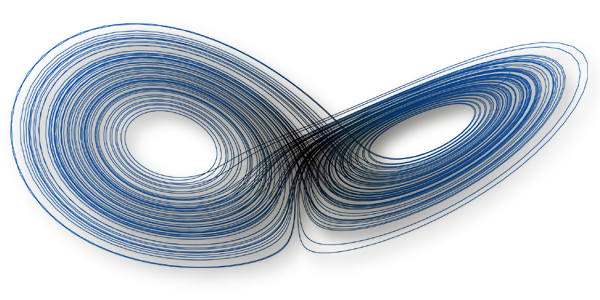
\includegraphics[width=.4\paperwidth]{cover.png}}

\date[unused]{ENSAM, Master 2, 2018--2019}

\begin{document}

\titleframe % Print the title as the first slide

%-------------------------------------------------------------------------------
%                           PRESENTATION SLIDES
%-------------------------------------------------------------------------------

% \begin{frame}[t, c]{}
% 	\centering
% 	\vspace{1cm}
%
% 	{\Large \textbf{First-order systems}}
%
% 	\bigskip
%
% 	{\textgre{\textbf{Flows on the line}}}
%
% \end{frame}

\begin{frame}[t, c]{Duffing oscillator}{A non-harmonic oscillator}
	\begin{itemize}
		\item Let us consider as an example the Duffing oscillator given by
		\begin{equation}
			\ddot{x} + \displaystyle \delta \dot{x} +  \alpha x  + \beta  x^3 = 0.
			\notag
		\end{equation}
		with $\alpha = -1$, $\beta = 1$ and $\delta = \nicefrac{1}{2}$.
		\bigskip

		\item It describes the motion of a damped oscillator with a more complex potential than simple harmonic motion.
		\begin{itemize}
			\item[$\hookrightarrow$] Example: a spring pendulum whose spring's stiffness does not exactly obey Hooke's law.
		\end{itemize}
	\end{itemize}

	\vspace{1cm}
\end{frame}

\begin{frame}[t, c]{Duffing oscillator}{A non-harmonic oscillator}
	\begin{itemize}
		\item Introducing $y = \dot{x}$, this second-order nonlinear ODE can be recast as a set of two first-order ODE with a nonlinear coupling term
		\begin{equation}
			\begin{aligned}
				\dot{x} & = y \\
				\dot{y} & = -\displaystyle \frac{1}{2} y +  x -  x^3.
			\end{aligned}
			\notag
		\end{equation}

		\bigskip

		\item Let us first discuss the different fixed points of the system.
	\end{itemize}

	\vspace{1cm}
\end{frame}

\begin{frame}[t, c]{Duffing oscillator}{Fixed points}
	\begin{itemize}
		\item The fixed points of the system are given by
		\begin{equation}
			\begin{aligned}
				y & = 0 \\
				x(1 - x^2) & = 0.
			\end{aligned}
			\notag
		\end{equation}

		\bigskip

		\item The system thus admits three different fixed points given by
		\medskip
		\begin{center}
			\begin{tabular}{ccc}
				$(x_1, y_1) = (0, 0)$ & $(x_2, y_2) = (1, 0)$ & $(x_3, y_3) = (-1, 0)$
			\end{tabular}
		\end{center}
	\end{itemize}

	\vspace{1cm}
\end{frame}

\begin{frame}[t, c]{Duffing oscillator}{Fixed points}
	\centering
	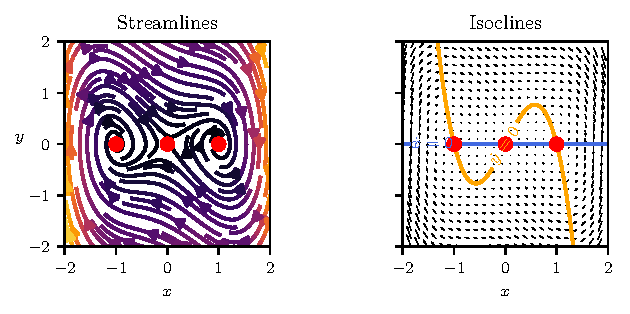
\includegraphics[width=.75\textwidth]{duffing_phase_plane}

	Phase plane and isoclines for the Duffing oscillator.

	\vspace{1cm}
\end{frame}

\begin{frame}[t, c]{Duffing oscillator}{Linear stability}
	\begin{itemize}
		\item The Jacobian matrix of the system reads
		\begin{equation}
			{\bm A}({\bm x}) = \begin{bmatrix}
									0 & 1 \\
									1 - 3x^2 & -0.5
								\end{bmatrix}
			\notag
		\end{equation}

		\bigskip

		\item As seen in the previous course, the linear stability of each fixed point ${\bm x}^*$ is governed by the eigenspectrum of ${\bm A}({\bm x}^*)$.
	\end{itemize}

	\vspace{1cm}
\end{frame}

\begin{frame}[t, c]{Duffing oscillator}{Linear stability}
	\begin{minipage}{.31\textwidth}
		\begin{block}{\centering ${\bm x}^*_1 = (0, 0)$}
			\bigskip
			\begin{itemize}
				\item Eigenvalues of ${\bm A}$ are
				$$\lambda_1 = 0.78$$
				and
				$$\lambda_2 = -1.28$$

				\item This fixed point is a \alert{\textbf{saddle}}.
			\end{itemize}
		\end{block}
	\end{minipage}%
	\hfill
	\begin{minipage}{.31\textwidth}
		\begin{block}{\centering ${\bm x}^*_2 = (1, 0)$}
			\bigskip
			\begin{itemize}
				\item Eigenvalues of ${\bm A}$ are
				$$\lambda_1 = -0.25 + 1.39 i$$
				and
				$$\lambda_2 = -0.25 - 1.39 i$$

				\item This fixed point is a \alert{\textbf{stable focus}}.
			\end{itemize}
		\end{block}
	\end{minipage}%
	\hfill
	\begin{minipage}{.31\textwidth}
		\begin{block}{\centering ${\bm x}^*_3 = (-1, 0)$}
			\bigskip
			\begin{itemize}
				\item Eigenvalues of ${\bm A}$ are
				$$\lambda_1 = -0.25 + 1.39 i$$
				and
				$$\lambda_2 = -0.25 - 1.39 i$$

				\item This fixed point is a \alert{\textbf{stable focus}}.
			\end{itemize}
		\end{block}
	\end{minipage}

	\vspace{1cm}
\end{frame}

\begin{frame}[t, c]{Duffing oscillator}{A dissipative dynamical system}
	\begin{itemize}
		\item Let us derive an equation for the total energy of the system
		\begin{equation}
			\dot{x} \left( \ddot{x} - x + x^3 \right) = - \displaystyle \frac{1}{2} \dot{x}
			\notag
		\end{equation}

		\bigskip

		\item After some simplification, this equation can be re-written as
		\begin{equation}
			\displaystyle \frac{\mathrm{d}}{\mathrm{d}t} \underbrace{\left[ \displaystyle \frac{1}{2} \left( \dot{x} \right)^2 - \frac{1}{2}x^2 + \frac{1}{4}x^4 \right]}_{\mathcal{H}} = - \frac{1}{2} \left( \dot{x} \right)^2,
			\notag
		\end{equation}
		where $\mathcal{H}$ is the total energy of the system.
	\end{itemize}

	\vspace{1cm}
\end{frame}

\begin{frame}[t, c]{Duffing oscillator}{A dissipative dynamical system}
	\begin{itemize}
		\item The governing equation for the total energy $\mathcal{H}$ finally reads
		$$\displaystyle \frac{\mathrm{d}}{\mathrm{d}t} \mathcal{H} = -\frac{1}{2} \left( \dot{x} \right)^2.$$

		\bigskip

		\item Clearly, as $t \to +\infty$, the total energy $\mathcal{H}$ tends to a constant value.
	\end{itemize}

	\bigskip

	\begin{block}{}
		\centering
		This is a \alert{\textbf{dissipative}} dynamical system.
	\end{block}

	\vspace{1cm}
\end{frame}

\begin{frame}[t, c]{Duffing oscillator}{A dissipative dynamical system}
	\centering
	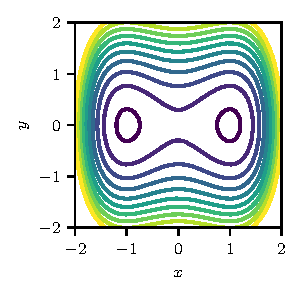
\includegraphics[width=.375\textwidth]{duffing_oscillator_potential}

	Isocontours of the total energy $\mathcal{H}$ of the Duffing oscillator.
\end{frame}

\begin{frame}[t, c]{Duffing oscillator}{}
	\centering

	\begin{block}{\centering \textbf{Question}}
		\centering
		Given an initial condition ${\bm x}_0$, toward which fixed point will it evolve as $t \to +\infty$?
	\end{block}

	\vspace{1cm}
\end{frame}

\begin{frame}[t, c]{Duffing oscillator}{Basin of attraction}
	\centering
	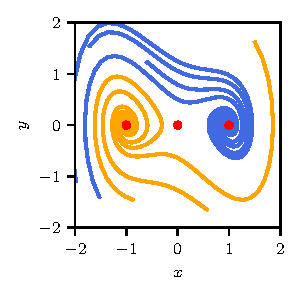
\includegraphics[width=.375\textwidth]{duffing_oscillator_basin}

	Trajectories of 8 randomly distributed initial conditions.

	\vspace{1cm}
\end{frame}

\begin{frame}[t, c]{Duffing oscillator}{Basin of attraction}
	\centering
	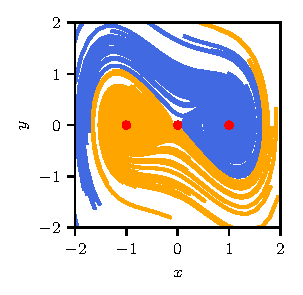
\includegraphics[width=.375\textwidth]{duffing_oscillator_basin_bis}

	Trajectories of 100 randomly distributed initial conditions.

	\vspace{1cm}
\end{frame}

\begin{frame}[t, c]{Duffing oscillator}{Basin of attraction}
	\begin{itemize}
		\item Not all initial conditions ${\bm x}_0$ end up to the same fixed point.

		\bigskip

		\item Two different regions appear well separated.
		\begin{itemize}
			\item[$\hookrightarrow$] These two regions are called the \alert{\textbf{basins of attraction}} of each fixed point.
		\end{itemize}

		\bigskip

		\item For the present dynamical system, a sharp frontier delimits these two regions. The saddle node ${\bm x}^*_1 = (0, 0)$ moreover appears to "sit" on this frontier.
	\end{itemize}

	\vspace{1cm}
\end{frame}

\begin{frame}[t, c]{Duffing oscillator}{Stable and unstable manifolds}
	\centering
	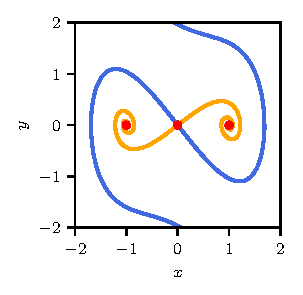
\includegraphics[width=.375\textwidth]{duffing_oscillator_saddle_manifold}

	Delimitation (blue) of the two basins of attraction.

	\vspace{1cm}
\end{frame}

\begin{frame}[t, c]{Duffing oscillator}{Stable and unstable manifolds}
	\centering
	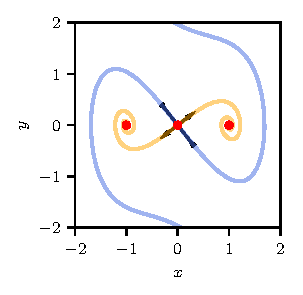
\includegraphics[width=.375\textwidth]{duffing_oscillator_saddle_manifold_bis}

	Arrows depict the linearly stable and unstable eigendirections of the saddle ${\bm x}^*_1 = (0, 0)$.

	\vspace{1cm}
\end{frame}

\begin{frame}[t, c]{Duffing oscillator}{Stable and unstable manifolds}
	\begin{itemize}
		\item On the previous plot, the blue line is called the \alert{\textbf{stable}} manifold ${\bm W}^s$ of ${\bm x}^*_1$, while the orange line is its \alert{\textbf{unstable}} manifold ${\bm W}^u$.

		\bigskip

		\item ${\bm W}^s$ and ${\bm W}^u$ are invariant sets, that is

		\bigskip

		\begin{quotation}
			An invariant set is a subset ${\bm W}$ of the phase space such that for any ${\bm x} \in {\bm W}$ and $t \in \mathbb{R}$, we have $\phi_t({\bm x}) \in {\bm W}$.
		\end{quotation}

		\bigskip

		\item Note that, if $\| {\bm x} \|$ is small enough, the stable (resp. unstable) manifold is tangent to the stable (resp. unstable) eigendirection of the fixed point.
	\end{itemize}

	\vspace{1cm}
\end{frame}

\begin{frame}[t, c]{Duffing oscillator}{Stable Manifold Theorem}
	\begin{block}{\textbf{Stable Manifold Theorem}}
		Suppose the origin is a fixed point of $\dot{\bm x} = f({\bm x})$. Let $E^s$ and $E^u$ be the sable and unstable subspaces of the linearization $\dot{x} = {\bm A}{\bm x}$, where ${\bm A}$ is the Jacobian matrix of $f$ at the origin. If $\| f({\bm x}) - {\bm A}{\bm x} \| = \mathcal{O}(\| {\bm x}\|^2)$, then $\exists$ \textbf{local stable and unstable manifolds} ${\bm W}_{loc}^s(0)$ and ${\bm W}_{loc}^u(0)$ which have the same dimension as $E^s$ and $E^u$ and are tangent to them at 0.
	\end{block}

	\vspace{1cm}
\end{frame}

\begin{frame}[t, c]{Duffing oscillator}{How to compute these manifolds?}
	\begin{block}{\centering \textbf{Brute force}}
	\end{block}

	\begin{itemize}
		\item Integrate numerically forward (resp. backward) in time an initial condition lying in the unstable (resp. stable) linear subspace of the fixed point.
	\end{itemize}

	\bigskip

	\begin{block}{\centering \textbf{Maths}}
	\end{block}

	\begin{itemize}
		\item Use Taylor expansion to compute an analytical expression of the stable and unstable manifolds.
	\end{itemize}

	\vspace{1cm}
\end{frame}

\begin{frame}[t, c]{Duffing oscillator}{How to compute these manifolds?}
	\begin{itemize}
		\item Let us assume that
		\begin{equation}
			\begin{aligned}
				y & = h(x) \\
				  & = a_1 x + a_2 x^2 + a_3 x^3 + \cdots \\
					& = \sum\limits_{k=1}^n a_k x^k.
			\end{aligned}
			\notag
		\end{equation}

		\bigskip

		\item Note moreover that
		\begin{equation}
			\dot{y} = \displaystyle \frac{\mathrm{d}x}{\mathrm{d}t} \frac{\mathrm{d}y}{\mathrm{d}x}
			\notag
		\end{equation}
	\end{itemize}

	\vspace{1cm}
\end{frame}

\begin{frame}[t, c]{Duffing oscillator}{How to compute these manifolds?}
	\begin{itemize}
		\item We then obtain that
		\begin{equation}
			\begin{aligned}
				\dot{y} & = h^{\prime}(x) \dot{x} \\
								& = \dot{x} \sum \limits_{k=1}^n a_k k x^{k-1}
			\end{aligned}
			\notag
		\end{equation}

		\bigskip

		\item By equating both sides, one obtains $n$ algebraic equations allowing us to determine the coefficients $a_k$ ($k= 1 \cdots n)$.
	\end{itemize}

	\vspace{1cm}
\end{frame}

\begin{frame}[t, c]{Duffing oscillator}{Application to our example}
	\begin{itemize}
		\item Let us compute cubic approximations of the stable and unstable manifolds of the saddle ${\bm x}^*_1 = (0, 0)$. We thus assume that
		\begin{equation}
			\begin{aligned}
				y & = h(x) \\
				  & = a x + b x^2 + c x^3. \\
			\end{aligned}
			\notag
		\end{equation}

		\bigskip

		\item Differentiating $h(x)$ with respect to $x$ gives
		$$h^{\prime}(x) = a + 2 b x + 3 c x^2.$$
	\end{itemize}

	\vspace{1cm}
\end{frame}

\begin{frame}[t, c]{Duffing oscillator}{Application to our example}
	\begin{itemize}
		\item Finally, we can write
		\begin{equation}
			\begin{aligned}
				h^{\prime}(x) \dot{x} - \dot{y} & = 0 \\
				h^{\prime}(x) y + \displaystyle \frac{1}{2}y - x + x^3 & = 0 \\
				(a + \displaystyle \frac{1}{2} + 2 b x + 3 c x^2) (a x + b x^2 + c x^3) - x + x^3 & = 0
			\end{aligned}
			\notag
		\end{equation}
	\end{itemize}

	\vspace{1cm}
\end{frame}

\begin{frame}[t, c]{Duffing oscillator}{Application to our example}
	\begin{itemize}
		\item After some calculations, we finally obtain that the coefficients in front of $x^k$ are solution to

		\medskip

		\begin{center}
			\begin{tabular}{ccc}
				$x$ & : & $a^2 + \displaystyle \frac{1}{2}a - 1 = 0$ \\
				$x^2$ & : & $\left( 3a + \displaystyle \frac{1}{2} \right) b = 0$ \\
				$x^3$ & : & $\left( 4a + \displaystyle \frac{1}{2} \right) c + 1= 0$
			\end{tabular}
		\end{center}

		\bigskip

		\item Finally, we obtain that the stable and unstable manifolds can be approximated by
		\begin{equation}
			h_{\pm}(x) = a_{\pm} x + c_{\pm} x^3.
			\notag
		\end{equation}
	\end{itemize}
\end{frame}

\begin{frame}[t, c]{Duffing oscillator}{Stable and unstable manifolds}
	\centering
	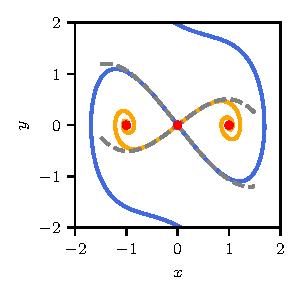
\includegraphics[width=.375\textwidth]{duffing_oscillator_saddle_manifold_ter}

	Dashed gray lines depict the poylnomial approximations of ${\bm W}^s$ and ${\bm W^u}$.

	\vspace{1cm}
\end{frame}

\begin{frame}[t, c]{}
	\centering
	\vspace{1cm}

	{\Large \textbf{Why do we bother with manifolds?}}

	\bigskip

	{\textgre{\textbf{A toy-model for subcritical transition to turbulence}}}

\end{frame}

\begin{frame}[t, c]{Subcritical transition to turbulence}{A toy-model}
	\begin{itemize}
		\item In 2014, Kerswell \emph{et al.}\ have proposed a simple toy-model to illustrate some aspect of subcritical transition to turbulence and so-called \emph{nonlinear optimal perturbations}.

		\bigskip

		\item This model reads
		\begin{equation}
			\begin{aligned}
				\dot{x} & = -x + 10y \\
				\dot{y} & = y(10e^{\nicefrac{-x^2}{100}} - y)(y -1).
			\end{aligned}
			\notag
		\end{equation}
	\end{itemize}

	\vspace{1cm}
\end{frame}

\begin{frame}[t, c]{Subcritical transition to turbulence}{A toy-model}
	\centering
	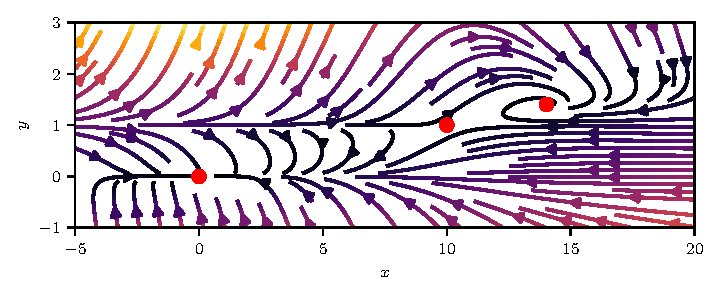
\includegraphics[width=.75\textwidth]{kerswell_phase_plane}

	Phase plane and fixed points of the toy-model considered.

	\vspace{1cm}
\end{frame}

\begin{frame}[t, c]{Subcritical transition to turbulence}{A toy-model}
	\centering

	The model admits three fixed points.

	\bigskip

	\begin{minipage}{.3\textwidth}
		\begin{block}{\centering \textbf{Laminar solution}}
		\end{block}
		\begin{itemize}
			\item ${\bm x}^*_1 = (0, 0)$
			\item Linearly stable sink.
		\end{itemize}
	\end{minipage}%
	\hfill
	\begin{minipage}{.3\textwidth}
		\begin{block}{\centering \textbf{The Edge}}
		\end{block}
		\begin{itemize}
			\item ${\bm x}^*_2 = (10, 1)$
			\item Saddle point.
		\end{itemize}
	\end{minipage}%
	\hfill
	\begin{minipage}{.3\textwidth}
		\begin{block}{\centering \textbf{Turbulent solution}}
		\end{block}
		\begin{itemize}
			\item ${\bm x}^* = (14.017, 1.4017)$
			\item Linearly stable focus.
		\end{itemize}
	\end{minipage}

	\vspace{1cm}
\end{frame}

\begin{frame}[t, c]{Subcritical transition to turbulence}{A toy-model}
	\centering
	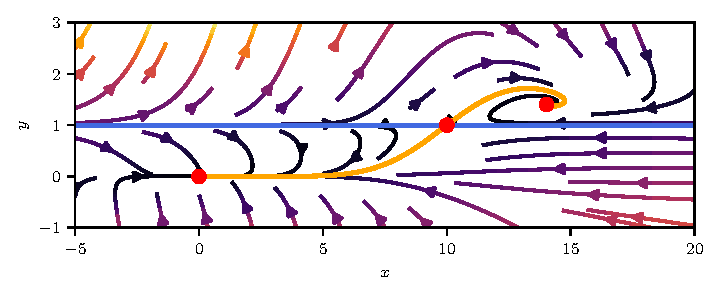
\includegraphics[width=.75\textwidth]{kerswell_phase_plane_bis}

	Stable (blue) and unstable (orange) manifolds of the Edge.

	\vspace{1cm}
\end{frame}

\begin{frame}[t, c]{Subcritical transition to turbulence}{A toy-model}
	\centering
	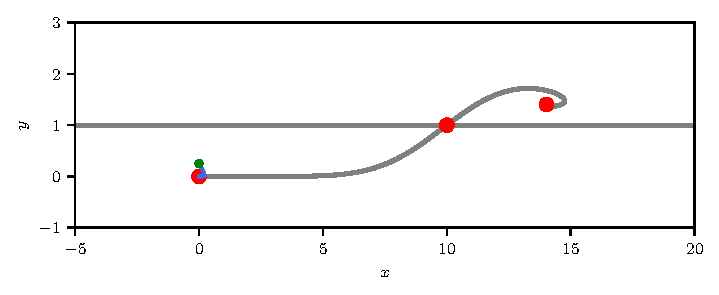
\includegraphics[width=.75\textwidth]{kerswell_phase_plane_ter_0}

	Trajectories for perturbations of different initial amplitude ($y_0 = 0.25, 0.5, 0.75, 0.999, 1.00001$).

	\vspace{1cm}
\end{frame}


\begin{frame}[t, c]{Subcritical transition to turbulence}{A toy-model}
	\centering
	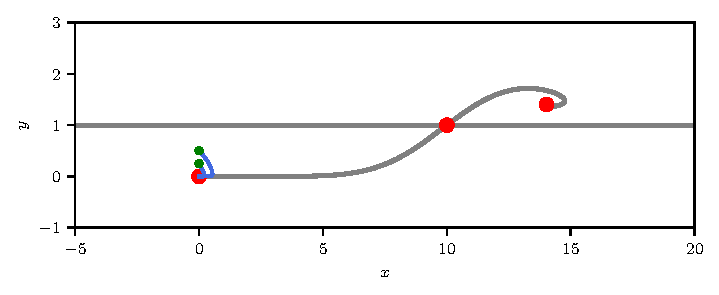
\includegraphics[width=.75\textwidth]{kerswell_phase_plane_ter_1}

	Trajectories for perturbations of different initial amplitude ($y_0 = 0.25, 0.5, 0.75, 0.999, 1.00001$).

	\vspace{1cm}
\end{frame}


\begin{frame}[t, c]{Subcritical transition to turbulence}{A toy-model}
	\centering
	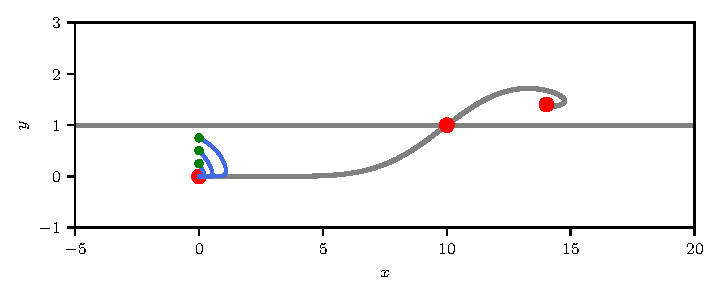
\includegraphics[width=.75\textwidth]{kerswell_phase_plane_ter_2}

	Trajectories for perturbations of different initial amplitude ($y_0 = 0.25, 0.5, 0.75, 0.999, 1.00001$).

	\vspace{1cm}
\end{frame}


\begin{frame}[t, c]{Subcritical transition to turbulence}{A toy-model}
	\centering
	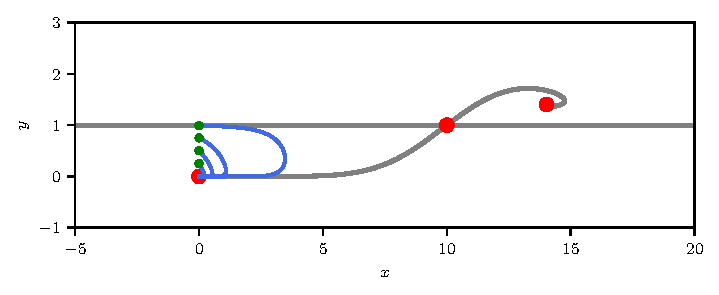
\includegraphics[width=.75\textwidth]{kerswell_phase_plane_ter_3}

	Trajectories for perturbations of different initial amplitude ($y_0 = 0.25, 0.5, 0.75, 0.999, 1.00001$).

	\vspace{1cm}
\end{frame}


\begin{frame}[t, c]{Subcritical transition to turbulence}{A toy-model}
	\centering
	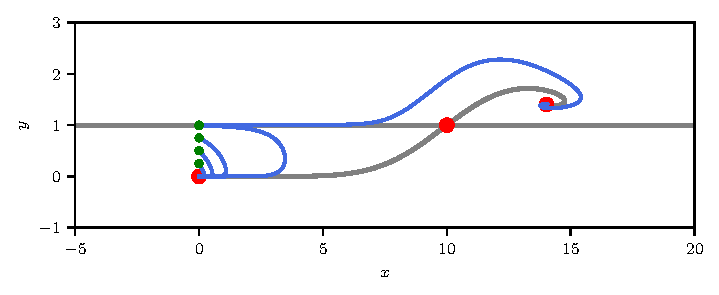
\includegraphics[width=.75\textwidth]{kerswell_phase_plane_ter_4}

	Trajectories for perturbations of different initial amplitude ($y_0 = 0.25, 0.5, 0.75, 0.999, 1.00001$).

	\vspace{1cm}
\end{frame}

\begin{frame}[t, c]{}
	\centering
	\vspace{1cm}

	{\Large \textbf{Exercises}}

	\bigskip

	{\textgre{\textbf{Do It Yourself}}}

\end{frame}

\begin{frame}[t, c]{Exercise}{A fairly simple example}
	\begin{itemize}
		\item Let us consider the following dynamical system
		\begin{equation}
			\begin{aligned}
				\dot{x} & = -x \\
				\dot{y} & = 2y - 5x^3.
			\end{aligned}
			\notag
		\end{equation}

		\bigskip

		\item You need to
		\begin{enumerate}
			\item Determine the fixed point of the system.
			\item Compute its linear stable and unstable eigenspaces.
			\item Compute an approximation of its stable and unstable manifolds.
		\end{enumerate}
	\end{itemize}

	\vspace{1cm}
\end{frame}

\begin{frame}[t, c]{Exercise}{A fairly simple example}
	\centering
	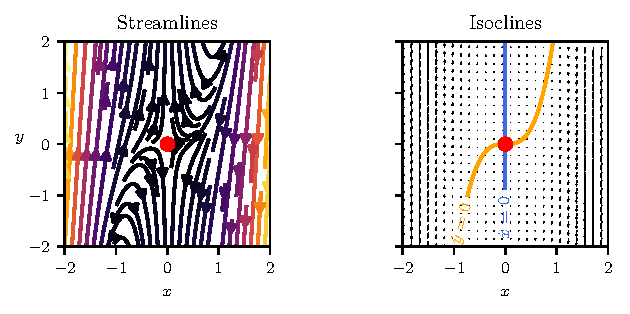
\includegraphics[width=.75\textwidth]{exercise_phase_plane}

	Phase plane and isoclines of the dynamical system considered.

	\vspace{1cm}
\end{frame}

\begin{frame}[t, c]{Another exercise}{A slightly more complex one}
	\begin{itemize}
		\item Let us now consider the following dynamical system
		\begin{equation}
			\begin{aligned}
				\dot{x} & = -x + y^2 \\
				\dot{y} & = y -x^2.
			\end{aligned}
			\notag
		\end{equation}

		\bigskip

		\item Do the same as before.
	\end{itemize}

	\vspace{1cm}
\end{frame}

\begin{frame}[t, c]{Exercise}{A slightly more complex one}
	\centering
	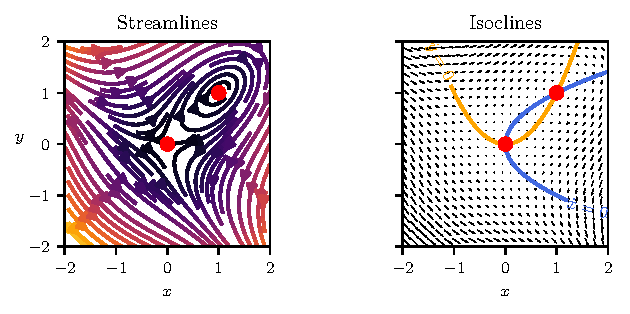
\includegraphics[width=.75\textwidth]{exercise_phase_plane_bis}

	Phase plane and isoclines of the dynamical system considered.

	\vspace{1cm}
\end{frame}

\end{document}
